\documentclass[aspectratio=169]{beamer}

\usetheme{Boadilla}
\usefonttheme{professionalfonts}
\setbeamertemplate{navigation symbols}{}
\setbeamertemplate{itemize items}[circle]
\setbeamertemplate{enumerate items}[default]
\setbeamertemplate{headline}{}

\usepackage[utf8]{inputenc}
\usepackage[T1]{fontenc}
\usepackage{lmodern}
\usepackage{amsmath}
\usepackage{booktabs}
\usepackage{tabularx}
\usepackage{array}
\usepackage{hyperref}
\usepackage[strings]{underscore}
\usepackage{listings}
\usepackage{tikz}
\usetikzlibrary{arrows.meta,positioning,fit,calc,shapes.geometric}
\usepackage{xcolor}

\definecolor{courseblue}{HTML}{12355B}
\definecolor{coursegold}{HTML}{C98A2E}
\definecolor{courseice}{HTML}{EEF3F8}
\definecolor{coursegreen}{HTML}{2F6B4F}
\definecolor{coursegray}{HTML}{4B5563}
\definecolor{codebg}{HTML}{F7F9FC}
\definecolor{codecomment}{HTML}{5E6C84}
\definecolor{codestring}{HTML}{0B6E4F}

\setbeamercolor{palette primary}{bg=courseblue,fg=white}
\setbeamercolor{palette secondary}{bg=coursegold,fg=white}
\setbeamercolor{palette tertiary}{bg=courseblue,fg=white}
\setbeamercolor{palette quaternary}{bg=coursegold,fg=white}
\setbeamercolor{structure}{fg=courseblue}
\setbeamercolor{frametitle}{bg=courseice,fg=courseblue}
\setbeamercolor{title}{fg=courseblue}
\setbeamercolor{block title}{bg=courseblue,fg=white}
\setbeamercolor{block body}{bg=courseice,fg=black}
\setbeamercolor{normal text}{fg=black,bg=white}
\setbeamercolor{alerted text}{fg=coursegold}

\setbeamerfont{footline}{size=\scriptsize}

\setbeamertemplate{footline}{
  \leavevmode
  \hbox{
    \begin{beamercolorbox}[wd=.33\paperwidth,ht=2.8ex,dp=1.2ex,leftskip=0.8em]{palette primary}%
      University of Trieste
    \end{beamercolorbox}%
    \begin{beamercolorbox}[wd=.49\paperwidth,ht=2.8ex,dp=1.2ex,center]{palette tertiary}%
      \coursename{} \textbar{} \coursecode
    \end{beamercolorbox}%
    \begin{beamercolorbox}[wd=.18\paperwidth,ht=2.8ex,dp=1.2ex,rightskip=0.8em plus1fil]{palette secondary}%
      \insertframenumber{} / \inserttotalframenumber
    \end{beamercolorbox}%
  }
}

\hypersetup{
  colorlinks=true,
  linkcolor=courseblue,
  urlcolor=coursegreen
}

\lstdefinestyle{coursepython}{
  language=Python,
  basicstyle=\ttfamily\footnotesize,
  keywordstyle=\color{courseblue}\bfseries,
  commentstyle=\color{codecomment}\itshape,
  stringstyle=\color{codestring},
  showstringspaces=false,
  columns=fullflexible,
  keepspaces=true,
  frame=single,
  framerule=0.6pt,
  rulecolor=\color{courseblue},
  backgroundcolor=\color{codebg},
  xleftmargin=0.4em,
  xrightmargin=0.4em,
  aboveskip=0.4em,
  belowskip=0.2em
}

\newcommand{\coursename}{Data-driven Systems Engineering}
\newcommand{\coursecode}{440MI / 305SM}
\newcommand{\coursefooter}{}

\newcommand{\learninggoals}[1]{
  \begin{block}{Learning goals}
  #1
  \end{block}
}

\newcommand{\repoactivity}[1]{
  \begin{block}{Repo activity}
  #1
  \end{block}
}

\newcommand{\readinglist}[1]{
  \begin{block}{Papers and materials}
  {\footnotesize #1}
  \end{block}
}

\newcommand{\coursecontextframe}[5]{
  \begin{frame}{Course Map and Running Cases}
  \centering
  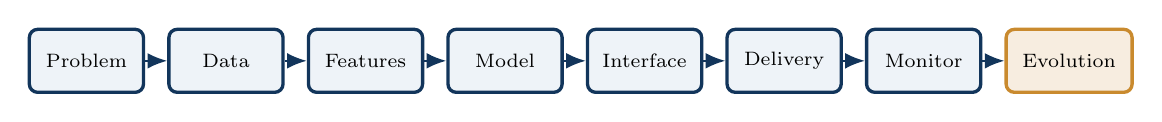
\begin{tikzpicture}[node distance=0.28cm]
  \node[flowbox, minimum width=1.45cm, minimum height=0.8cm] (problem) {\scriptsize Problem};
  \node[flowbox, minimum width=1.45cm, minimum height=0.8cm, right=of problem] (data) {\scriptsize Data};
  \node[flowbox, minimum width=1.45cm, minimum height=0.8cm, right=of data] (features) {\scriptsize Features};
  \node[flowbox, minimum width=1.45cm, minimum height=0.8cm, right=of features] (model) {\scriptsize Model};
  \node[flowbox, minimum width=1.45cm, minimum height=0.8cm, right=of model] (interface) {\scriptsize Interface};
  \node[flowbox, minimum width=1.45cm, minimum height=0.8cm, right=of interface] (delivery) {\scriptsize Delivery};
  \node[flowbox, minimum width=1.45cm, minimum height=0.8cm, right=of delivery] (monitor) {\scriptsize Monitor};
  \node[accentbox, minimum width=1.6cm, minimum height=0.8cm, right=of monitor] (evolution) {\scriptsize Evolution};
  \foreach \a/\b in {problem/data,data/features,features/model,model/interface,interface/delivery,delivery/monitor,monitor/evolution} {
    \draw[arrow] (\a) -- (\b);
  }
  \end{tikzpicture}

  \vspace{0.5em}
  \begin{block}{Today in the course}
  \textbf{Focus:} #1

  \textbf{Bridge:} #2
  \end{block}

  \begin{columns}[T]
  \column{0.48\textwidth}
  \begin{block}{Fraud case}
  {\footnotesize #3}
  \end{block}
  \column{0.48\textwidth}
  \begin{block}{Pasteurization case}
  {\footnotesize #4}
  \end{block}
  \end{columns}

  \vspace{0.3em}
  {\footnotesize \textbf{Course thread:} #5}
  \coursefooter
  \end{frame}
}

\newcommand{\classclosingframe}[4]{
  \begin{frame}{From This Class to the Next}
  \begin{block}{What stays with us}
  #1
  \end{block}

  \begin{columns}[T]
  \column{0.48\textwidth}
  \begin{block}{Project use}
  {\footnotesize #2}
  \end{block}
  \column{0.48\textwidth}
  \begin{block}{Next connection}
  {\footnotesize #3}
  \end{block}
  \end{columns}

  \vspace{0.3em}
  {\footnotesize \textbf{Course thread:} #4}
  \coursefooter
  \end{frame}
}

\tikzset{
  flowbox/.style={
    rounded corners=3pt,
    draw=courseblue,
    fill=courseice,
    very thick,
    minimum width=2.2cm,
    minimum height=0.9cm,
    align=center,
    font=\small
  },
  accentbox/.style={
    rounded corners=3pt,
    draw=coursegold,
    fill=coursegold!15,
    very thick,
    minimum width=2.2cm,
    minimum height=0.9cm,
    align=center,
    font=\small
  },
  arrow/.style={
    -{Latex[length=2.5mm,width=2mm]},
    thick,
    draw=courseblue
  }
}


\title{Class 13: MLOps Foundations and Production Readiness}
\author{\coursename}
\date{}

\begin{document}

\frame{\titlepage \coursefooter}

\begin{frame}{Agenda}
\begin{itemize}
\item AI maturity and why adoption is hard
\item Overview of MLOps
\item Workflow, lifecycle processes, infrastructure, and roles
\item Preparing for production
\item What maturity looks like in this repository
\end{itemize}
\coursefooter
\end{frame}

\begin{frame}{MLOps is coordination under change}
\learninggoals{
\begin{itemize}
\item Define MLOps as the integration of model development with operational discipline.
\item Understand the roles and handoffs involved in production ML.
\item Evaluate whether a project is production-ready or only demo-ready.
\item Distinguish DevOps concerns from additional MLOps concerns.
\end{itemize}
}
\coursefooter
\end{frame}

\coursecontextframe
{Operational ownership across the ML lifecycle.}
{This class connects engineering artifacts to production responsibilities, showing how data, models, services, and monitoring become one operating system.}
{In the fraud case, MLOps means reproducible training, artifact versioning, safe deployment, and monitoring for score shift and analyst load.}
{In the pasteurization case, MLOps means streaming behavior, drift detection, rollback thinking, and operational visibility for process anomalies.}
{This is the point where the course unifies software engineering, experimentation, delivery, and monitoring into one lifecycle.}

\begin{frame}{Why MLOps became necessary}
\begin{itemize}
\item Training a model is only one part of delivering value.
\item Organizations discovered that models fail at the boundaries: data access, packaging, deployment, monitoring, and ownership.
\item MLOps formalizes the work needed to make ML systems reproducible, operable, and governable.
\end{itemize}
\begin{block}{Core idea}
MLOps is not a single tool. It is a coordination discipline supported by automation, standards, and clear responsibility.
\end{block}
\coursefooter
\end{frame}

\begin{frame}{Why AI adoption is hard}
\begin{itemize}
\item Excessive manual work across teams.
\item Fragile handoffs from data engineering to modeling to deployment.
\item Missing standards for experiments, artifacts, and rollback.
\item Poor visibility into model behavior after release.
\end{itemize}
\coursefooter
\end{frame}

\begin{frame}{Common failure points in ML adoption}
\begin{itemize}
\item A model works in a notebook but cannot be rebuilt consistently.
\item Data and feature assumptions are undocumented.
\item Deployment ownership is unclear between data, software, and ops teams.
\item Monitoring starts after launch instead of before launch.
\item Governance appears only when something has already gone wrong.
\end{itemize}
\coursefooter
\end{frame}

\begin{frame}{AI maturity view}
\begin{itemize}
\item Early stage: isolated experiments and manual deployment.
\item Emerging stage: repeatable training and some CI/CD.
\item Managed stage: monitoring, governance, and clearer role boundaries.
\item Scaled stage: standardized pipelines, traceability, and controlled retraining.
\end{itemize}
\coursefooter
\end{frame}

\begin{frame}{What maturity changes in practice}
\begin{tabularx}{\textwidth}{>{\bfseries}l X}
Maturity signal & What it means \\
\toprule
Repeatable experiments & Teams can reproduce a result from code, data, and config. \\
Versioned artifacts & A deployed model can be traced and rolled back. \\
Automated delivery & Packaging and validation happen consistently. \\
Monitoring and alerts & Teams detect failure before users must explain it. \\
Governed retraining & Change happens through a controlled path, not by accident. \\
\bottomrule
\end{tabularx}
\coursefooter
\end{frame}

\begin{frame}{Where MLOps adds work beyond DevOps}
\begin{itemize}
\item Data versioning and validation.
\item Experiment tracking and model registry.
\item Training, retraining, and rollback logic.
\item Monitoring for data, model, and business behavior.
\item Governance for fairness, auditability, and safe access.
\end{itemize}
\coursefooter
\end{frame}

\begin{frame}{DevOps versus MLOps}
\begin{columns}[T]
\column{0.48\textwidth}
\textbf{DevOps focus}
\begin{itemize}
\item Build and release software safely
\item Reliability, scaling, observability
\item Infrastructure and deployment automation
\end{itemize}
\column{0.48\textwidth}
\textbf{MLOps additions}
\begin{itemize}
\item Data and feature validation
\item Training and retraining workflows
\item Model registry, drift, and evaluation governance
\end{itemize}
\end{columns}
\coursefooter
\end{frame}

\begin{frame}{A practical MLOps lifecycle}
\begin{enumerate}
\item Frame the business question and success criteria.
\item Acquire, validate, and document data.
\item Train and compare candidate models.
\item Package the winning artifact and dependencies.
\item Validate through tests and release gates.
\item Deploy with observability.
\item Monitor, diagnose, and decide on retraining or rollback.
\end{enumerate}
\coursefooter
\end{frame}

\begin{frame}{MLOps workflow}
\centering
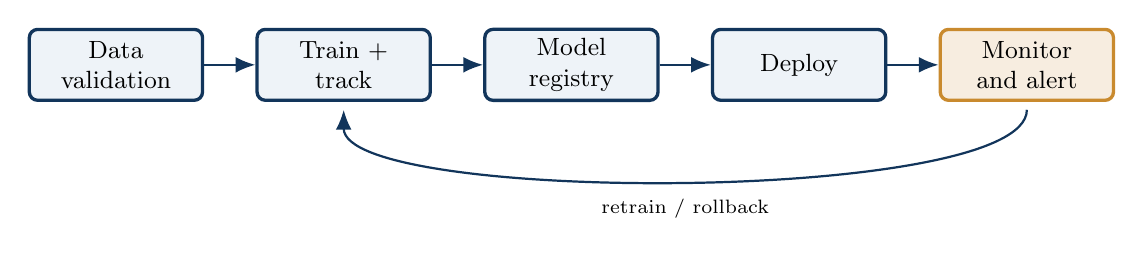
\begin{tikzpicture}[node distance=0.65cm and 0.65cm]
\node[flowbox] (data) {Data\\validation};
\node[flowbox, right=of data] (train) {Train +\\track};
\node[flowbox, right=of train] (registry) {Model\\registry};
\node[flowbox, right=of registry] (deploy) {Deploy};
\node[accentbox, right=of deploy] (monitor) {Monitor\\and alert};
\draw[arrow] (data) -- (train);
\draw[arrow] (train) -- (registry);
\draw[arrow] (registry) -- (deploy);
\draw[arrow] (deploy) -- (monitor);
\draw[arrow] ($(monitor.south)+(0,-0.10)$)
  .. controls +(0,-1.20) and +(0,-1.20) ..
  node[below, font=\scriptsize, yshift=-0.10cm] {retrain / rollback}
  ($(train.south)+(0,-0.10)$);
\end{tikzpicture}
\coursefooter
\end{frame}

\begin{frame}{Infrastructure layers behind the workflow}
\begin{itemize}
\item Storage layer: raw data, features, models, logs.
\item Compute layer: notebooks, training jobs, CI runners, containers.
\item Serving layer: APIs, dashboards, schedulers, or streaming components.
\item Observability layer: metrics, logs, drift detection, alerts, dashboards.
\item Governance layer: permissions, approvals, lineage, and audit records.
\end{itemize}
\coursefooter
\end{frame}

\begin{frame}{Roles around the lifecycle}
\centering
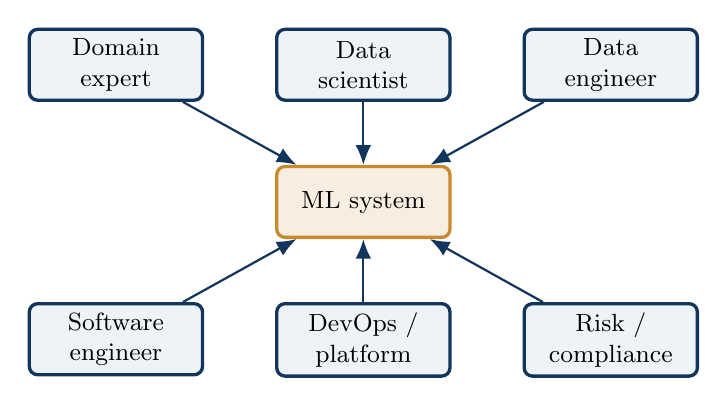
\begin{tikzpicture}[node distance=0.8cm and 0.9cm]
\node[accentbox] (core) {ML system};
\node[flowbox, above left=of core] (domain) {Domain\\expert};
\node[flowbox, above=of core] (ds) {Data\\scientist};
\node[flowbox, above right=of core] (de) {Data\\engineer};
\node[flowbox, below left=of core] (se) {Software\\engineer};
\node[flowbox, below=of core] (ops) {DevOps /\\platform};
\node[flowbox, below right=of core] (risk) {Risk /\\compliance};
\foreach \n in {domain,ds,de,se,ops,risk} {
  \draw[arrow] (\n) -- (core);
}
\end{tikzpicture}
\vspace{0.5em}
\begin{itemize}
\item MLOps is mostly about reducing friction across these handoffs.
\end{itemize}
\coursefooter
\end{frame}

\begin{frame}{Typical handoffs that create friction}
\begin{itemize}
\item Data engineering to data science: access, freshness, schema meaning.
\item Data science to software engineering: artifact packaging, interfaces, dependencies.
\item Software engineering to operations: deployment behavior, scaling, secrets, rollback.
\item Operations back to the ML team: incidents, drift, and degraded outcomes.
\end{itemize}
\begin{block}{Lesson}
If a team cannot explain its handoffs, it is probably not ready for dependable production work.
\end{block}
\coursefooter
\end{frame}

\begin{frame}{A practical production-readiness checklist}
\begin{itemize}
\item Can we rebuild the model from code, data, and config?
\item Can we explain which version is running and why?
\item Do we know how the service fails and who is notified?
\item Is there a monitoring plan before launch?
\item Do stakeholders agree on success and rollback criteria?
\end{itemize}
\coursefooter
\end{frame}

\begin{frame}{Demo-ready versus production-ready}
\begin{columns}[T]
\column{0.48\textwidth}
\textbf{Demo-ready}
\begin{itemize}
\item Works on one machine
\item Manual execution
\item Little failure handling
\item Monitoring absent or superficial
\end{itemize}
\column{0.48\textwidth}
\textbf{Production-ready}
\begin{itemize}
\item Reproducible environment
\item Versioned artifacts and configs
\item Clear ownership and rollback path
\item Monitoring and operational evidence
\end{itemize}
\end{columns}
\coursefooter
\end{frame}

\begin{frame}{Repo-aligned maturity example}
\repoactivity{
The repository already spans multiple maturity stages: exploratory notebooks, serialized artifacts, Flask APIs, Streamlit dashboards, and CI/CD tutorials. This makes it a strong teaching example for the transition from experimentation to operations.
}
\coursefooter
\end{frame}

\begin{frame}{How this repository illustrates MLOps}
\begin{itemize}
\item `notebooks/` shows early-stage exploration and model building.
\item `pasteurization/` and `streamlit/` show how behavior becomes a service or interface.
\item `tutorials/Docker`, `tutorials/GitHubActions`, and `tutorials/Jenkins` show operationalization paths.
\item Monitoring examples in `App_Stream.py` connect deployed behavior to feedback and drift response.
\end{itemize}
\coursefooter
\end{frame}

\classclosingframe
{\begin{itemize}
\item MLOps connects experimentation, packaging, release, monitoring, and ownership into one lifecycle.
\item The hard part is not only training a model but keeping it reliable after handoff.
\item Operational maturity comes from repeatability, observability, and clear responsibilities.
\end{itemize}}
{This is the lens teams can now use to evaluate whether their project behaves like an engineered system or only like an isolated analysis artifact.}
{Class 14 turns that lifecycle view into project proposals, milestones, and execution plans for a complete semester project.}
{The course now moves from concepts and tools into explicit planning for how a team will deliver and defend its own system.}

\begin{frame}{Papers and materials}
\readinglist{
\href{https://research.google/pubs/pub46555/}{Sculley et al., Hidden Technical Debt in Machine Learning Systems};\ 
\href{https://www.oreilly.com/library/view/practical-mlops/9781098103002/}{Practical MLOps};\ 
\href{https://www.oreilly.com/library/view/designing-machine-learning/9781098107956/}{Designing Machine Learning Systems};\ 
\href{https://cloud.google.com/architecture/mlops-continuous-delivery-and-automation-pipelines-in-machine-learning}{Google Cloud MLOps guidance};\ 
\href{https://neptune.ai/blog/mlops-best-practices}{MLOps best practices overview};\ 
\href{https://evidentlyai.com/ml-observability}{ML observability materials from Evidently}.
}
\coursefooter
\end{frame}

\end{document}
